\section{Methodology}
\label{sec:method}

Our analysis follows the evidence from a constituent query to its composed counterpart. We first identify the heads whose bridge access changes when the bridge becomes implicit, then read out the address information they retain. We next separate paragraph access from local token weighting to measure their interaction. Finally, we use the localized heads and address signals in \method\ (\cref{fig:causal_framework,fig:framework}).

\subsection{Paired Contextual Reasoning}
\label{sec:triplets}
For a fact chain $e_0\xrightarrow{r_1}b\xrightarrow{r_2}a$, each source pairs the composed question $q_{12}$ with two constituent questions: $q_1$ asks for bridge $b$, and $q_2$ explicitly names $b$ and asks for answer $a$. The paragraph about $e_0$ is the \emph{root paragraph}; the paragraph supporting $(b,r_2,a)$ is the \emph{bridge paragraph}. All three queries share the original evidence, including its supporting sentences, distractors, and paragraph positions. The pair $(q_2,q_{12})$ therefore asks for the same endpoint through explicit and implicit formulations of the bridge.

Let $c_i(q)\in\{0,1\}$ denote correctness for source $i$. Following the conditional compositionality gap \citep{press2023compositionality}, the native constituent-correct set is $\mathcal U=\{i:c_i(q_1)c_i(q_2)=1\}$, and its composition failure rate is
\begin{equation}
  \mathrm{CFR}=1-\frac{1}{|\mathcal U|}\sum_{i\in\mathcal U}c_i(q_{12}).
  \label{eq:cfr}
\end{equation}
This population lets us measure composition failures despite correct answers to both constituent questions. We also report composed accuracy over all sources and all-three accuracy, which requires both constituent answers and the composed answer to be correct. Repair rates use the original native population throughout.

\subsection{Localizing Evidence-Access Heads}
\label{sec:localize}
\textbf{Head ranking.} For attention head $h$ at layer $\ell$, let $A^{\ell h}_{t,k}$ be attention from question token $t$ to context token $k$. Its mass on paragraph $p_j$ is $m^{\ell h}_t(j)=\sum_{k\in p_j}A^{\ell h}_{t,k}$. We rank heads on paired discovery queries by
\begin{equation}
  d_{\ell h}=\E_i\!\left[\bar m^{\ell h}_{q_2}(j_i^*)-
  \bar m^{\ell h}_{q_{12}}(j_i^*)\right],
  \label{eq:ranking}
\end{equation}
where $j_i^*$ is the annotated bridge and $\bar m$ averages question-token rows. A large score identifies a head that allocates more attention to the bridge when it is explicitly named. We select the head count using discovery-set mass calibration: among $20/40/80$ heads, we choose the count with the highest composed accuracy and prefer the smaller set on a tie. This yields 20, 20, and 40 heads for Qwen3-4B, Qwen3-8B, and Llama-3.1-8B. Setting their outputs to zero at question-prefill positions, alongside layer-matched random knockout, measures their causal contribution to answering.

\textbf{Recovering bridge addresses.} To determine whether the selected heads retain the location of the next fact, we fit a linear paragraph scorer $s_j=w^\top f_j$. Each head contributes two features: the log mean question-token mass and the log last-question-token mass on paragraph $j$. The full scorer also includes log paragraph-to-prompt token ratio and a question/title-mention indicator. Attention-only and metadata-only variants measure the information supplied by each feature group. Feature standardization and paragraph-index cross-entropy training with $\ell_2$ regularization use the 2,000 composed training examples. The native-state readout measures address recoverability during failures; a separately fitted readout on adapted-model features is used in \method\ (Appendix~\ref{app:readout_protocol}).

\begin{figure*}[!t]
  \centering
  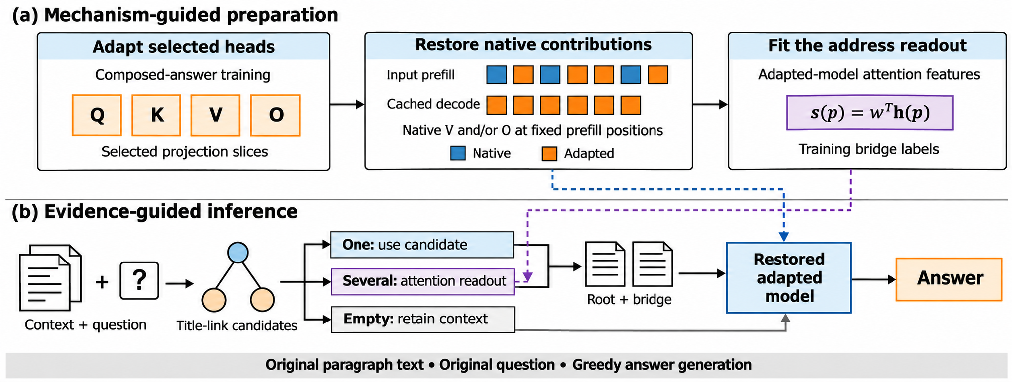
\includegraphics[width=\textwidth]{figures/figure3_method.pdf}
  \caption{\textbf{Overview of CoReTrace.} Offline, selected Q/K/V/O slices are adapted, fixed prefill rules restore native V/O contributions, and the training-fitted address reader is prepared. At inference, a title graph supplies candidate paragraphs. A unique candidate is selected directly; ambiguous candidates trigger the frozen readout. The root and selected bridge retain their original text and order. Inapplicable graphs retain the full context.}
  \label{fig:framework}
\end{figure*}

\subsection{Separating Access from Local Reading}
\label{sec:factorization}
Attention to a paragraph combines two quantities: how much of the row reaches that paragraph, and how that mass is distributed over its tokens. For bridge paragraph $B$, write $m=\sum_{k\in B}A_k$ and $\rho_k=A_k/m$, so $A_k=m\rho_k$ and $\sum_{k\in B}\rho_k=1$. We call $m$ the \emph{access mass} and $\rho$ the \emph{local reading pattern}. The paragraph's contribution before the output projection is
\begin{equation}
  c_B=m\sum_{k\in B}\rho_k v_k.
  \label{eq:contribution}
\end{equation}
Here $v_k$ is the value vector computed by the receiving model \citep{vaswani2017attention}. The factor $m$ scales the contribution of the paragraph, while $\rho$ determines the relative contribution of its token values. This factorization supplies two separately controllable quantities for studying how evidence access shapes reading.

\textbf{Crossed attention intervention.} We cross two access settings with two local patterns (\cref{fig:causal_framework}b). Native $(m,\rho)$ retains the composed query's attention. Mass $(\tau,\rho)$ calibrates paragraph access while preserving its local pattern. Pattern $(m,\rho^{\rm dir})$ transfers the direct query's local pattern while preserving native access. Both $(\tau,\rho^{\rm dir})$ combines the two changes. The contrast asks whether the same direct-query pattern has a different effect at the two access levels.

Each head's target $\tau$ is its mean last-token bridge mass on direct discovery queries. The donor supplies the normalized bridge pattern at the paired direct query's final question token, transferred to every selected receiver question row. Outside-bridge attention is rescaled to preserve the row total. All arms use receiver-computed values and the original output-projection weights; subsequent activations and caches follow the intervened forward pass.

To align donor and receiver evidence, we construct 25 discovery quadruplets that cross two bridges with two second-hop relations in a common ten-paragraph context. The 100 composed receivers and their paired direct queries have identical context-token positions. We quantify the dependence of the pattern effect on access using
\begin{equation}
 I=\mathrm{Acc}_{\mathrm{both}}-\mathrm{Acc}_{\mathrm{mass}}
 -\mathrm{Acc}_{\mathrm{pattern}}+\mathrm{Acc}_{\mathrm{native}}
 \label{eq:interaction}
\end{equation}
Thus, $I$ is the pattern effect under calibrated access minus its effect under native access. We obtain paired intervals by resampling quadruplets, keeping all queries and intervention arms in a shared context together. A complementary experiment applies the same frozen access targets to the bridge, root, or a length-matched other paragraph on the test panel. This measures how the effect depends on the destination of access. Appendix~\ref{app:interventions} specifies the transformations and implementation checks.

\subsection{CoReTrace: Mechanism-Guided Repair}
\label{sec:repair}
The analysis identifies both a set of heads that mediate evidence access and address information that can guide evidence selection. \method\ uses these findings to focus the model's input and adapt the computation of the selected heads (\cref{fig:framework}).

\textbf{Selected-head adaptation.} We train full-rank query, key, value, and output (Q/K/V/O) projection slices in the localized heads using answer-only cross-entropy, with all other model parameters frozen. Fixed projection restoration reinstates native V and/or O contributions at designated prompt-prefill positions, combining native prefill contributions with adapted computation; cached decoding uses the adapted weights. The model-specific scopes are fixed before the reported evaluation suite (\cref{tab:scopes}).

\textbf{Attention-guided evidence selection.} Paragraph titles mentioned in the question identify the root when exactly one title is independently matched. Other paragraph titles appearing in the root's body define candidate bridges. A unique candidate is selected directly; multiple candidates trigger one full-context prefill under the adapted/restored model, whose address readout ranks them by $s_j$. The root and highest-scoring bridge are then supplied to the model in their original wording and order. Inputs without an applicable candidate graph retain the complete context. Inference uses the question, paragraph texts, and frozen model and readout parameters.
